\documentclass[aspectratio=169]{beamer}

\mode<presentation>

\usepackage[utf8]{inputenc}
\usepackage[T1]{fontenc}	%makes å,ä,ö etc. proper symbols
\usepackage{amsmath}
\usepackage{graphicx}
\usepackage{xcolor}
\usepackage{listings}
\usepackage{multicol}
\usepackage{hyperref}
\usepackage[swedish]{babel}

\definecolor{LundaGroen}{RGB}{00,68,71}
\definecolor{StabilaLila}{RGB}{85,19,78}
\definecolor{VarmOrange}{RGB}{237,104,63}

\definecolor{MagnoliaRosa}{RGB}{251,214,209}
\definecolor{LundaHimmel}{RGB}{204,225,225}
\definecolor{LundaLjus}{RGB}{255,242,191}

\usefonttheme{serif}
\usetheme{malmoe}
\setbeamercolor{palette primary}{bg=LundaHimmel, fg=StabilaLila}
\setbeamercolor{palette quaternary}{bg=LundaGroen, fg=MagnoliaRosa}
\setbeamercolor{background canvas}{bg=LundaLjus}
\setbeamercolor{structure}{fg=LundaGroen}

\usepackage[many]{tcolorbox}

\newtcolorbox{cross}{blank,breakable,parbox=false,
  overlay={\draw[red,line width=5pt] (interior.south west)--(interior.north east);
    \draw[red,line width=5pt] (interior.north west)--(interior.south east);}}
    
\newcommand{\code}[1]{\colorbox{white}{\lstinline{#1}}}



\lstset{language=Python} 
\lstset{%language=[LaTeX]Tex,%C++,
    morekeywords={PassOptionsToPackage,selectlanguage,True,False},
    keywordstyle=\color{blue},%\bfseries,
    basicstyle=\small\ttfamily,
    %identifierstyle=\color{NavyBlue},
    commentstyle=\color{red}\ttfamily,
    stringstyle=\color{VarmOrange},
    numbers=left,%
    numberstyle=\scriptsize,%\tiny
    stepnumber=1,
    numbersep=8pt,
    showstringspaces=false,
    breaklines=true,
    %frameround=ftff,
    frame=single,
    belowcaptionskip=.75\baselineskip,
	tabsize=4,
	backgroundcolor=\color{white}
    %frame=L
}


\begin{document}

\lstset{literate=
  {á}{{\'a}}1 {é}{{\'e}}1 {í}{{\'i}}1 {ó}{{\'o}}1 {ú}{{\'u}}1
  {Á}{{\'A}}1 {É}{{\'E}}1 {Í}{{\'I}}1 {Ó}{{\'O}}1 {Ú}{{\'U}}1
  {à}{{\`a}}1 {è}{{\`e}}1 {ì}{{\`i}}1 {ò}{{\`o}}1 {ù}{{\`u}}1
  {À}{{\`A}}1 {È}{{\'E}}1 {Ì}{{\`I}}1 {Ò}{{\`O}}1 {Ù}{{\`U}}1
  {ä}{{\"a}}1 {ë}{{\"e}}1 {ï}{{\"i}}1 {ö}{{\"o}}1 {ü}{{\"u}}1
  {Ä}{{\"A}}1 {Ë}{{\"E}}1 {Ï}{{\"I}}1 {Ö}{{\"O}}1 {Ü}{{\"U}}1
  {â}{{\^a}}1 {ê}{{\^e}}1 {î}{{\^i}}1 {ô}{{\^o}}1 {û}{{\^u}}1
  {Â}{{\^A}}1 {Ê}{{\^E}}1 {Î}{{\^I}}1 {Ô}{{\^O}}1 {Û}{{\^U}}1
  {œ}{{\oe}}1 {Œ}{{\OE}}1 {æ}{{\ae}}1 {Æ}{{\AE}}1 {ß}{{\ss}}1
  {ű}{{\H{u}}}1 {Ű}{{\H{U}}}1 {ő}{{\H{o}}}1 {Ő}{{\H{O}}}1
  {ç}{{\c c}}1 {Ç}{{\c C}}1 {ø}{{\o}}1 {å}{{\r a}}1 {Å}{{\r A}}1
  {€}{{\euro}}1 {£}{{\pounds}}1 {«}{{\guillemotleft}}1
  {»}{{\guillemotright}}1 {ñ}{{\~n}}1 {Ñ}{{\~N}}1 {¿}{{?`}}1
}

\AtBeginSection[ ]
{
\begin{frame}{Innehåll}
    	\tableofcontents[currentsection]
\end{frame}
}

\title{Felmeddelanden}
\date{ht 22}
\author{Programmering 1}

\maketitle

\section{Introduktion}

\subsection{Vilka stöter vi på?}

\begin{frame}
\frametitle{Felmeddelanden}

När vi kör vår kod riskerar vi att få följande felmeddelanden:

\begin{itemize}
\item \texttt{NameError}
\item \texttt{IndexError}
\item \texttt{TypeError}
\item \texttt{SyntaxError}
\item \texttt{UnboundLocalError}
\end{itemize}

Det finns självfallet fler. Man kan till och med göra sina egna.

\end{frame}

\subsection{Hur ser det ut?}

\begin{frame}[fragile]
\frametitle{Felmeddelandet}

\begin{lstlisting}[language=, style=]
Traceback (most recent call last):
  File "\\intra.lund.se\userdata\071837\Kurser\Programmering\1819\Sankaskepp\sankaskepp.py", line 175, in <module>
    träff = kollaträff(gissning[0], gissning[1])
  File "\\intra.lund.se\userdata\071837\Kurser\Programmering\1819\Sankaskepp\sankaskepp.py", line 125, in kollaträff
    hej
NameError: name 'hej' is not defined
\end{lstlisting}

\end{frame}

\section{Felmeddelanden}

\subsection{Odefinierad variabel}

\begin{frame}[fragile]
\frametitle{NameError}
\framesubtitle{Odefinierad variabel}

\begin{lstlisting}
b = a+5
\end{lstlisting}

\begin{lstlisting}[style=,language=]
Traceback (most recent call last):
  File "<pyshell#12>", line 1, in <module>
    b=a+5
NameError: name 'a' is not defined
\end{lstlisting}

Här försöker vi använda variabeln \texttt{a} innan den är skapad.

\end{frame}

\subsection{Fel index}

\begin{frame}[fragile]
\frametitle{IndexError}
\framesubtitle{Fel i listor}

\begin{lstlisting}
lista = [6,4,2]
print(lista[5])
\end{lstlisting}

\begin{lstlisting}[style=, language=]
Traceback (most recent call last):
  File "<pyshell#1>", line 1, in <module>
    lista[5]
IndexError: list index out of range
\end{lstlisting}

Det här felet uppstår när man vill komma åt ett för stort index i listan.

\end{frame}

\subsection{Funktionsanrop}

\begin{frame}[fragile]
\frametitle{TypeError}
\framesubtitle{Fel antal argument}

\begin{lstlisting}
for i in range():
    print(i)
\end{lstlisting}

\begin{lstlisting}[language=,style=]
Traceback (most recent call last):
  File "<pyshell#5>", line 1, in <module>
    for i in range():
TypeError: range expected 1 arguments, got 0
\end{lstlisting}

Här har vi skickat in för få argument/parametrar till funktionen. Man kan också få samma meddelande om man skickar in för många.

\end{frame}

\subsection{Ogiltiga operationer}

\begin{frame}[fragile]
\frametitle{TypeError}
\framesubtitle{Okompatibla operationer}

\begin{lstlisting}
5+[0,2]
\end{lstlisting}

\begin{lstlisting}[language=,style=]
Traceback (most recent call last):
  File "<pyshell#8>", line 1, in <module>
    5+[0,2]
TypeError: unsupported operand type(s) for +: 'int' and 'list'
\end{lstlisting}

Här har vi försökt addera ett tal med en lista vilket Python inte förstår. Man får ett liknande fel om man skriver något i stil med \texttt{5+''hej''}.

\end{frame}

\begin{frame}[fragile]
\frametitle{TypeError}
\framesubtitle{Okompatibla operationer}

\begin{lstlisting}
[0,2]+5
\end{lstlisting}

\begin{lstlisting}[language=,style=]
Traceback (most recent call last):
  File "<pyshell#9>", line 1, in <module>
    [0,2]+5
TypeError: can only concatenate list (not "int") to list
\end{lstlisting}

Här har vi försökt addera slå ihop en lista och ett tal vilket Python inte förstår. Det blir likadant om man försöker sig på något i stil med \texttt{''hej''+5}.

\end{frame}

\subsection{Syntax}

\begin{frame}[fragile]
\frametitle{SyntaxError}
\framesubtitle{Tecken-fel}

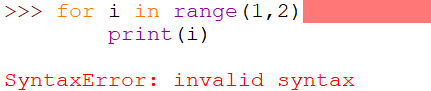
\includegraphics[width=0.8\textwidth]{SyntaxError1.png}

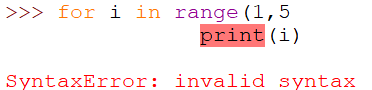
\includegraphics[width=0.7\textwidth]{SyntaxError2.png}

Om man missar ett tecken får man ett SyntaxError. Missar man parantesen så kommer felet att visas på raden nedanför. Det finns andra sätt att få SyntaxError också, men gemensamt är att det är ett fel som gör det omöjligt för programmet att tolka koden.

\end{frame}

\begin{frame}[fragile]
\frametitle{SyntaxError}
\framesubtitle{Missad indentering}

\begin{lstlisting}
if 2<3:
print(5)
\end{lstlisting}

\begin{lstlisting}[language=,style=]
SyntaxError: expected an indented block
\end{lstlisting}

\end{frame}

\subsection{''Odefinerad''}

\begin{frame}[fragile]
\frametitle{UnboundLocalError}

\begin{lstlisting}
a=3
def func():
    a+=1
    return a
\end{lstlisting}

\begin{lstlisting}[style=,language=]
Traceback (most recent call last):
  File "<pyshell#30>", line 1, in <module>
    func()
  File "<pyshell#29>", line 2, in func
    a+=1
UnboundLocalError: local variable 'a' referenced before assignment
\end{lstlisting}

Här har vi försökt skriva till variabeln \texttt{a} utan att ha deklarerat den inuti funktionen.

\end{frame}

\section{Övningar}

\begin{frame}
	\frametitle{Övningar}
	
	Ladda ner filen \texttt{felmeddelanden.py} från Classroom och lös alla felmeddelanden.
	
	
\end{frame}

\end{document}